\documentclass[aspectratio=169,11pt]{beamer}
\usepackage[spanish,es-nodecimaldot]{babel}
\usepackage{amsmath,amssymb,booktabs}
\usepackage{graphicx}
\usepackage{xcolor}
\usepackage{hyperref}

\definecolor{Ink}{HTML}{17212B}
\definecolor{Blue}{HTML}{176B87}
\definecolor{Coral}{HTML}{D65A4A}
\definecolor{Paper}{HTML}{F7F4EE}
\definecolor{Gray}{HTML}{66717C}
\setbeamercolor{normal text}{fg=Ink,bg=Paper}
\setbeamercolor{frametitle}{fg=Ink,bg=Paper}
\setbeamercolor{title}{fg=Ink}
\setbeamercolor{structure}{fg=Blue}
\setbeamercolor{alerted text}{fg=Coral}
\setbeamertemplate{navigation symbols}{}
\setbeamertemplate{itemize item}{\color{Blue}\raise0.2ex\hbox{\small$\blacksquare$}}
\setbeamertemplate{frametitle}{\vspace{0.45cm}\insertframetitle\par\vspace{-0.1cm}\color{Blue}\rule{\textwidth}{1.2pt}}
\setbeamertemplate{footline}{\hfill\color{Gray}\scriptsize\insertframenumber\hspace{0.35cm}\vspace{0.22cm}}
\newcommand{\source}[1]{\vfill{\color{Gray}\tiny Fuente: #1}}
\newcommand{\key}[1]{{\color{Coral}\bfseries #1}}

\title{Delegación agéntica y frontera de lenguajes}
\subtitle{Una reconstrucción crítica de Quispe y Xu (2026)}
\author{sbvasquezg-ux}
\date{Septiembre de 2026}

\begin{document}

\begin{frame}[plain]
  \vspace{0.7cm}
  {\usebeamerfont{title}\color{Ink}\LARGE\inserttitle\par}
  \vspace{0.25cm}
  {\Large\color{Blue}\insertsubtitle\par}
  \vfill
  {\large\insertauthor\par}
  \vspace{0.18cm}
  {\small\href{https://github.com/sbvasquezg-ux/ai-03-quispe}{github.com/sbvasquezg-ux/ai-03-quispe}\par}
  \vspace{0.35cm}
  {\small\insertdate\par}
\end{frame}

\begin{frame}{La pregunta económica}
  \Large
  ¿Un asistente que \key{ejecuta} tareas amplía el conjunto de lenguajes en los que una persona puede producir?

  \vspace{0.8cm}
  \normalsize
  El contraste relevante del paper es un cambio de menú:
  \[
  \underbrace{\{\text{solo},\text{conversación}\}}_{M_1}
  \quad\longrightarrow\quad
  \underbrace{\{\text{solo},\text{conversación},\text{delegación}\}}_{M_2}.
  \]
  La frontera es de \emph{producción}, no de habilidad adquirida.
  \source{Quispe y Xu, secciones 3--4.2 y Remark 1, PDF pp. 10--17.}
\end{frame}

\begin{frame}{El problema del agente}
  Para cada desarrollador, lenguaje y mes:
  \[
  m^g\in\arg\max_{m\in M_g\cup\{\varnothing\}}\{V^m,0\},
  \qquad Z^g=\mathbf1\{\max_{m\in M_g}V^m\ge0\}.
  \]
  \small
  \[
  \begin{aligned}
  V^S&=\omega+s\mu-\frac{\rho s^2}{2\pi}-b,\\
  V^C&=V^S+\gamma s-r_C,\\
  V^D&=\omega+(1-\lambda)s\mu+\lambda az(A)-\kappa-r_D-b\\
  &\hspace{1.8cm}-\frac{\rho}{2}\left[\frac{(1-\lambda)^2s^2}{\pi}+\sigma_D^2\right].
  \end{aligned}
  \]
  \source{Sección 4.1, ecuaciones 1--3, PDF pp. 13--14. Reconstrucción separable del programa.}
\end{frame}

\begin{frame}{La decisión que lo separa de ALZ}
  \begin{columns}[T,onlytextwidth]
    \column{0.47\textwidth}
    \textbf{Aouad--Lykouris--Zhong}

    \vspace{0.2cm}
    Margen intensivo continuo:
    \[
    x=s+e+a.
    \]
    La IA sustituye skill y esfuerzo dentro de una tarea.

    \column{0.47\textwidth}
    \textbf{Quispe--Xu}

    \vspace{0.2cm}
    Margen extensivo discreto:
    \[
    Z^g=\mathbf1\{\omega\ge T^g\}.
    \]
    La delegación añade un modo y puede abrir un lenguaje.
  \end{columns}

  \vspace{0.55cm}
  \key{La diferencia formal es el umbral de entrada específico por lenguaje.}
  \source{Quispe y Xu, sección 4.2, PDF pp. 14--16. ALZ: formulación semanal de referencia.}
\end{frame}

\begin{frame}{Proposición 2: todas las condiciones}
  \small
  Sea un lenguaje \textbf{no familiar}. Bajo el Supuesto 1,
  \(\gamma s-r_C\le0\), entonces \(T^1=T^S\). Defina
  \[
  T^S=b-s\mu+\frac{\rho s^2}{2\pi},\qquad B=T^S-T^D.
  \]
  Si \(B>0\),
  \[
  \boxed{Z^2-Z^1=\mathbf1\{T^D\le\omega<T^S\}}.
  \]
  Si además la CDF condicional \(F\) es continua,
  \[
  \Pr(Z^2-Z^1=1)=F(T^S)-F(T^D),\qquad
  E[N^2-N^1]\ge0.
  \]
  Expansión estricta exige masa positiva dentro de alguna banda. Continuidad sola no basta.
  \source{Proposición 2 y ecuaciones 4--9, PDF pp. 14--16.}
\end{frame}

\begin{frame}{Qué mueve la agencia}
  \[
  \begin{aligned}
  B={}&\lambda[az(A)-s\mu]-\kappa(a,s)-r_D\\
  &+\frac{\rho}{2}\left[\frac{(2\lambda-\lambda^2)s^2}{\pi}-\sigma_D^2(a,s,A)\right].
  \end{aligned}
  \]
  \begin{itemize}
    \item Sustituye ejecución humana por competencia del agente.
    \item Cambia el riesgo del match y añade error residual.
    \item Añade verificación y cómputo.
  \end{itemize}
  Pero los outcomes observan solamente el resultado reducido: \key{cuánto cayó el umbral}.
  \source{Ecuación 7 y discusión, sección 4.2, PDF p. 15.}
\end{frame}

\begin{frame}{Modelo rival: el mismo umbral sin agente}
  Un shock genérico \(q\ge0\) reduce el costo efectivo de entrada:
  \[
  \widetilde T=T^S-q,
  \qquad \widetilde Z-Z^1=\mathbf1\{T^S-q\le\omega<T^S\}.
  \]
  Si \(F\) tiene densidad \(f\),
  \[
  P(q)=F(T^S)-F(T^S-q),\qquad P'(q)=f(T^S-q)\ge0.
  \]
  Elegir \(q=B\) replica la banda agéntica. Permitir \(q=q(a,s,A)\) replica también las comparativas por habilidad.

  \vspace{0.35cm}
  \key{Sin una comparación chat versus agente, “agéntico” no queda identificado por estos outcomes.}
  \source{Modelo rival y derivación propios; contraste con ecuaciones 7--9 del paper.}
\end{frame}

\begin{frame}{Evidencia que sí elimina explicaciones mecánicas}
  \centering
  \begin{tabular}{lrr}
    \toprule
    ATT en \(e=0\) & Baseline & Robustez \\
    \midrule
    Lenguajes activos & 2.528 & 1.580 sin lenguaje inicial \\
    Lenguajes nuevos & 1.193 & 0.807 sin lenguaje inicial \\
    Lenguajes activos & 2.528 & 1.663 sin trailer Claude \\
    \bottomrule
  \end{tabular}

  \vspace{0.65cm}
  Linguist excluye JSON, YAML, markup, data, vendored, generated y documentation. La contaminación existe, pero no explica todo el patrón.
  \source{Sección 5.3, PDF p. 22; tablas 3--4, PDF pp. 37--39.}
\end{frame}

\begin{frame}{La selección que sobrevive}
  \begin{itemize}
    \item Sí hay controles not-yet-treated y placebo doce meses antes.
    \item Conteo mensual y flujo nuevo tienen pre-periodos planos.
    \item El stock acumulado falla: cuatro de cinco pre-coeficientes son significativos.
    \item Actividad y lenguajes ya aumentan en \(e=-1\).
  \end{itemize}
  \vspace{0.35cm}
  Un proyecto nuevo puede causar a la vez adopción y diversificación. Mover \(e=-1\) a la ventana de anticipación no hace exógeno el timing.

  \vspace{0.35cm}
  \key{El diseño identifica event time, no causalidad ni mecanismo.}
  \source{Secciones 6.1, 7.1--7.3, 8.6 y 10.2--10.7, PDF pp. 25--26, 31--33, 44, 50--53.}
\end{frame}

\begin{frame}{Especialistas: mecanismo o reversión a la media}
  Los primeros usos crecen más entre especialistas dentro de cada mitad de actividad:
  \[
  0.98\;\text{vs.}\;0.30\quad(\text{alta actividad}),\qquad
  2.39\;\text{vs.}\;1.02\quad(\text{baja actividad}).
  \]
  El doble ordenamiento corrige parte de la medición por volumen, pero no el \emph{headroom} mecánico: quien parte cerca de cero tiene más lenguajes que pueden contar como nuevos.

  \vspace{0.35cm}
  Test faltante: estimar la tasa de descubrimiento esperada sin adopción para personas emparejadas en actividad, breadth e historia larga; idealmente, asignar agente versus chat al azar.
  \source{Tabla 7 y sección 9, PDF pp. 45--49; nota 4 sobre historia desde 2024, PDF p. 22.}
\end{frame}

\begin{frame}{Lean: la frontera de la traducción}
  \textbf{(a) Proposición original}
  \[
  \Delta C_i(s)=\sum_{k\in U_i}\left[(1-p^1_{ik})^{s+1}-(1-p^2_{ik})^{s+1}\right].
  \]
  El paper afirma crecimiento y concavidad estrictos si \(p^1=0<p^2\).

  \textbf{(b) Enunciado Lean y prueba}

  \texttt{PENDIENTE: el workflow no generó archivos Lean.}

  \texttt{check} falló en Python 3.9 antes de cargar el paper. No existe un fragmento de prueba que pueda mostrarse sin fabricarlo.

  \textbf{(c) Qué debía verificar}

  Dominios de hazards, no-vacuidad de \(U_i\), desigualdad estricta y endpoint \(p^2=1\). El bloqueo está documentado en \texttt{lean/PENDIENTE.md}.
  \source{Proposición 3, PDF p. 17; prueba A.6, PDF pp. 63--64. Registro local de EconCSLib.}
\end{frame}

\begin{frame}{El endpoint que rompe la Proposición 3}
  Tome un solo lenguaje no familiar:
  \[
  U_i=\{k\},\qquad p^1_{ik}=0,\qquad p^2_{ik}=1.
  \]
  Entonces, para todo \(s\ge0\),
  \[
  \Delta C_i(s)=1^{s+1}-0^{s+1}=1.
  \]
  La primera diferencia vale cero. El paso
  \[
  p^2(1-p^2)^{s+1}>0
  \]
  falla exactamente en \(p^2=1\). Reparación: \(0<p^2<1\) y al menos un candidato no familiar relevante.
  \source{Proposición 3 y apéndice A.6, PDF pp. 17 y 63--64. Contraejemplo propio reproducido en sim.py.}
\end{frame}

\begin{frame}{Dónde no le creí a la IA}
  \begin{columns}[T,onlytextwidth]
    \column{0.53\textwidth}
    \small
    \textbf{Comprobación manuscrita}

    \vspace{0.2cm}
    \IfFileExists{hand/prop3-endpoint.jpg}{
      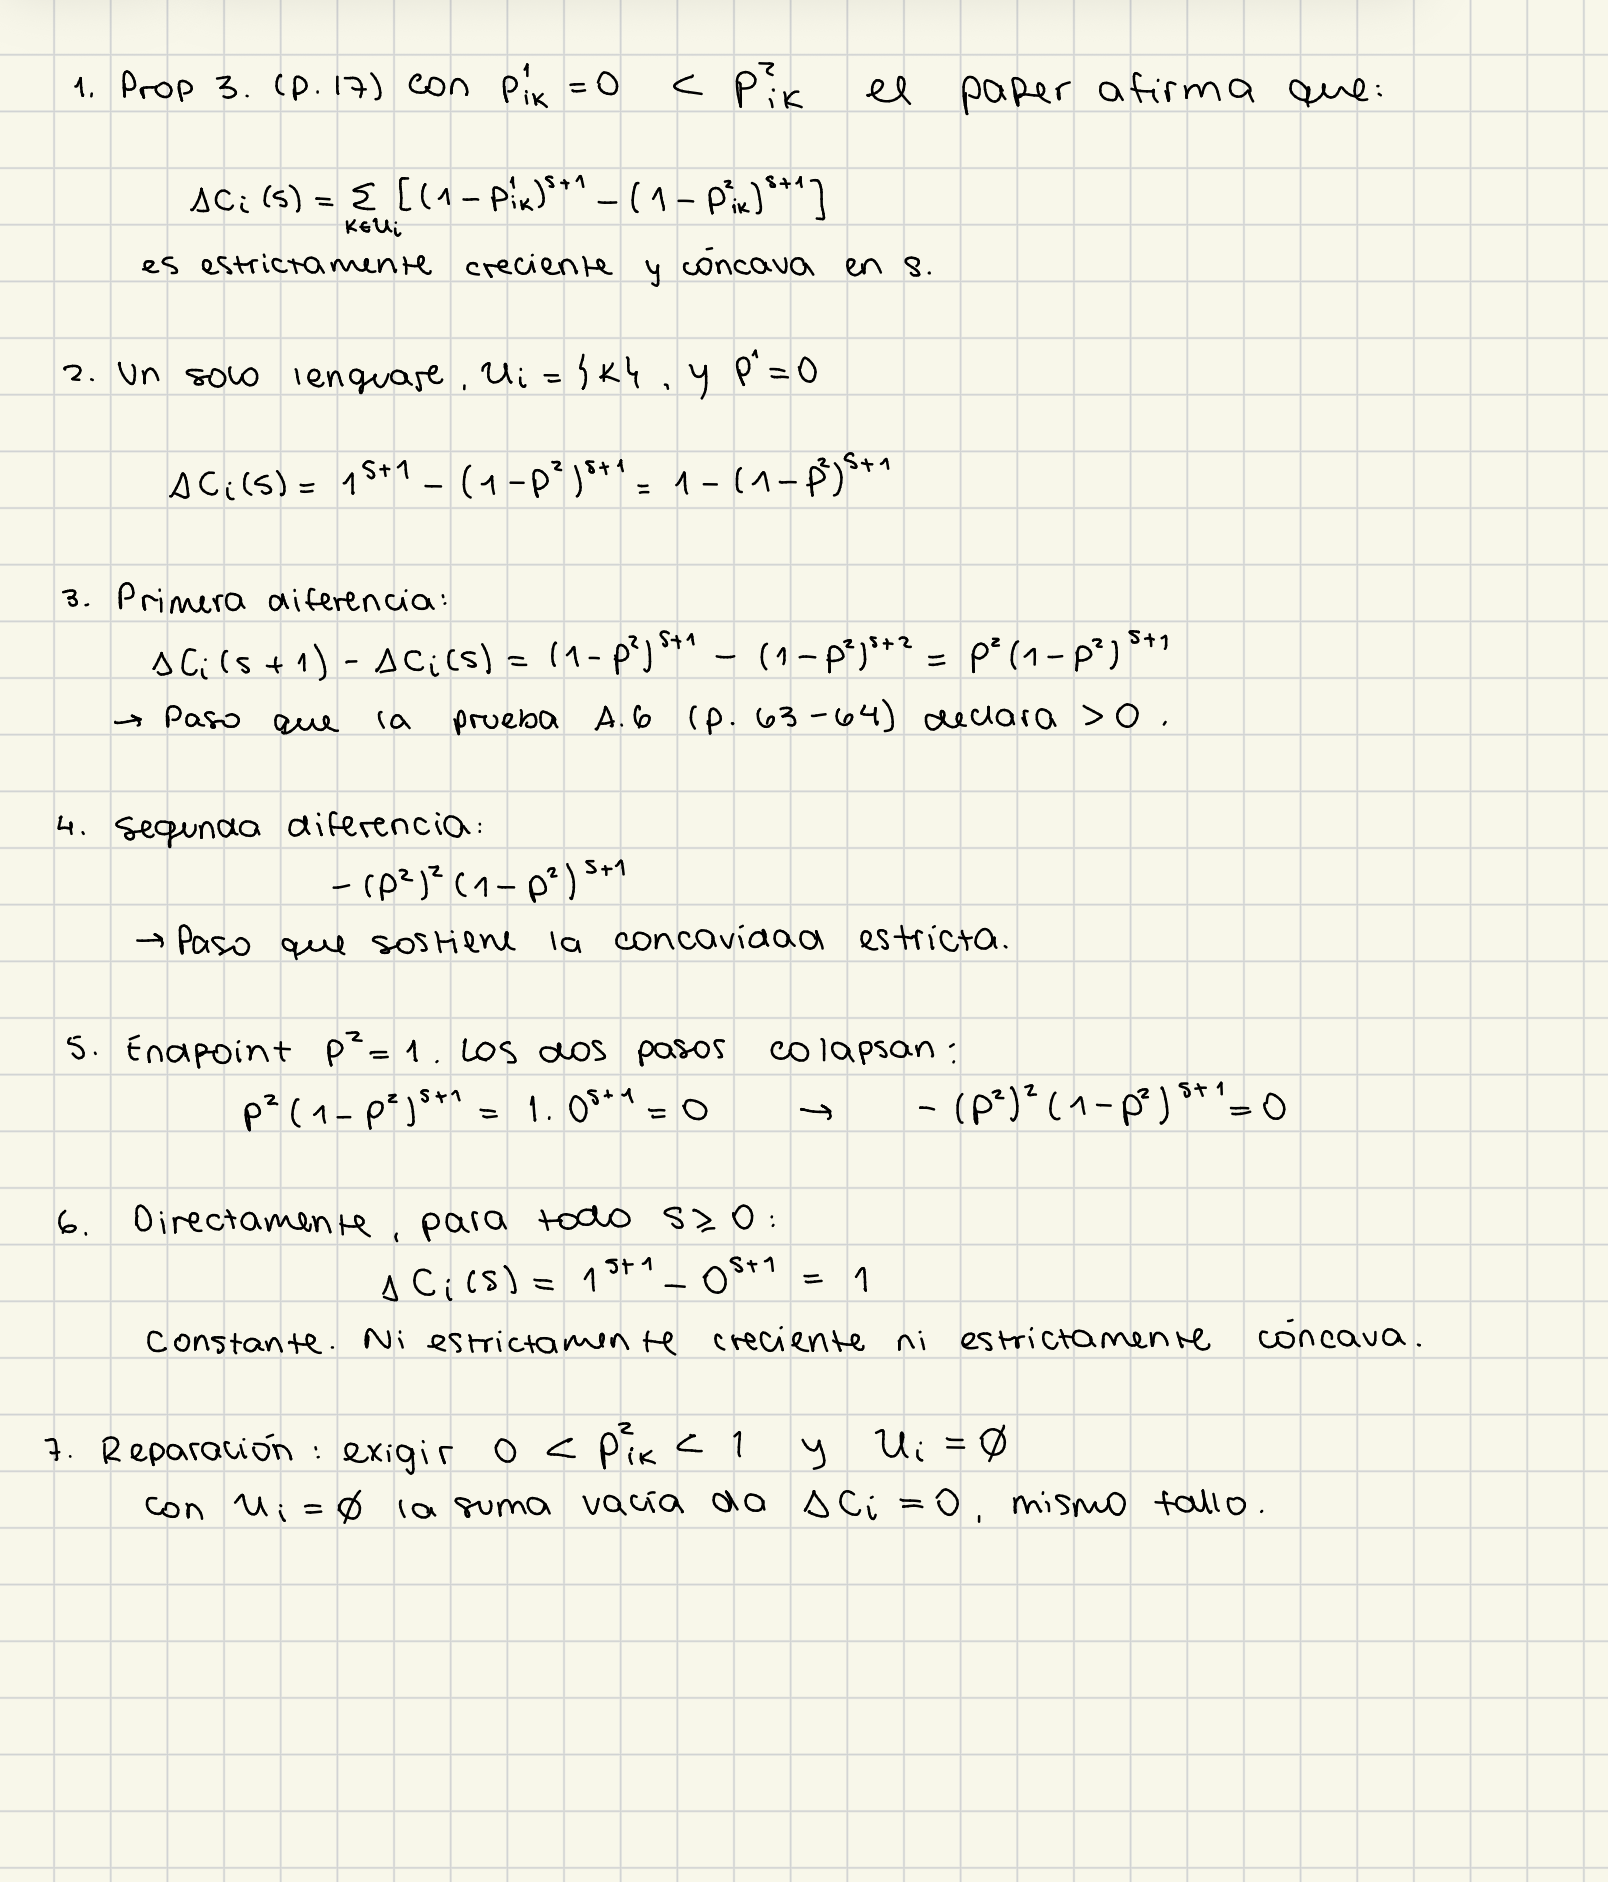
\includegraphics[width=\linewidth,height=0.56\textheight,keepaspectratio]{hand/prop3-endpoint.jpg}
    }{
      \IfFileExists{hand/prop3-endpoint.png}{
        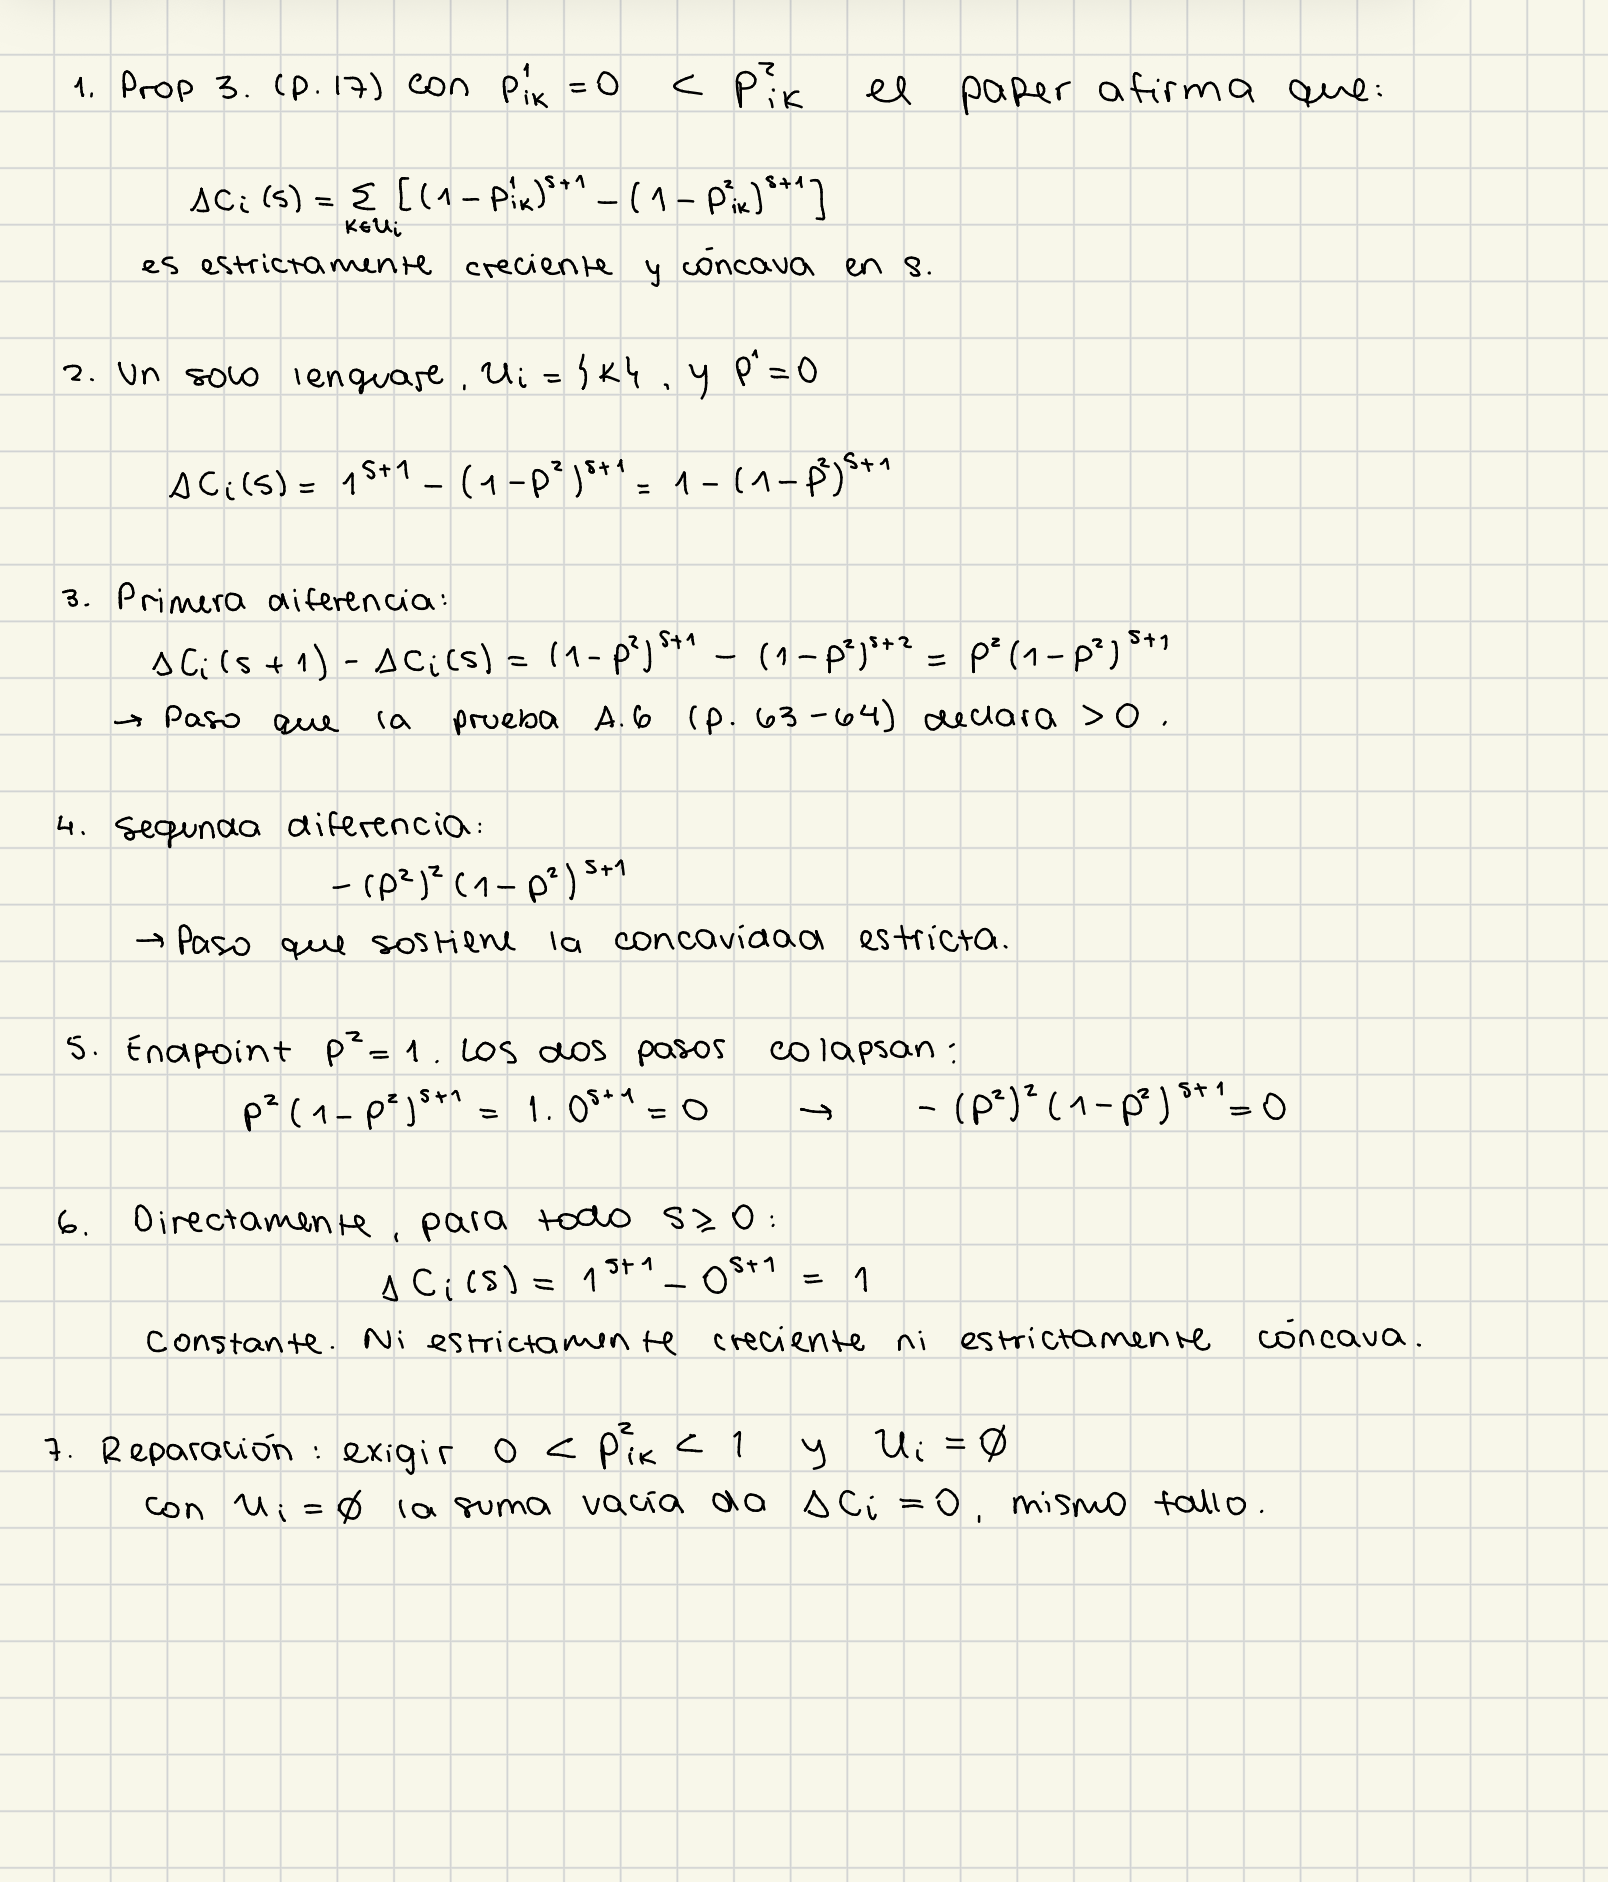
\includegraphics[width=\linewidth,height=0.56\textheight,keepaspectratio]{hand/prop3-endpoint.png}
      }{
        \fbox{\parbox[c][0.45\textheight][c]{0.92\linewidth}{\centering Foto real pendiente\\[0.4cm]\texttt{hand/prop3-endpoint.jpg}}}
      }
    }

    \column{0.42\textwidth}
    \textbf{Veredicto}

    \vspace{0.3cm}
    La asociación es sólida frente a varias contaminaciones observables.

    \vspace{0.35cm}
    La causalidad no está identificada.

    \vspace{0.35cm}
    La agencia tampoco: un shock genérico puede mover el mismo umbral.

    \vspace{0.35cm}
    Una desigualdad estricta del modelo falla en un endpoint permitido.
  \end{columns}
  \source{Análisis propio; framing causal del paper en sección 10.7, PDF p. 53.}
\end{frame}

\begin{frame}{Qué sobrevive}
  \Large
  La primera coautoría detectable de Claude coincide con una expansión grande y transitoria del portafolio de producción.

  \vspace{0.6cm}
  \normalsize
  Es consistente con la activation band, pero también con selección por proyecto y con un shock genérico de productividad. El experimento decisivo compara chat y agente manteniendo constante el modelo base y asignando el acceso exógenamente.

  \vfill
  \color{Blue}\large
  La objeción no elimina el hecho descriptivo. Limita el salto desde ese hecho hacia causalidad y mecanismo.
  \source{Quispe y Xu, secciones 10.2--10.7, PDF pp. 50--53; modelo rival propio.}
\end{frame}

\end{document}
